\section{Anomalous Quartic Gauge Couplings}
\label{sec:aqgc_limit}

The sensitivity of this analysis to the anomalous quartic gauge coupling
(aQGC) signal described in \sec\ref{sec:eft} and 
\sec\ref{sec:aqgc_signal} has also been assessed.  This aQGC signal predicts
more events than the SM alone. Since the measurement of the SM signal in
\sec\ref{sec:measurement} was shown to be consistent with the data, this implies
that no aQGC signal has been observed. However, we can set a limit on the sensitivity 
to this signal.

In this section we first describe the prediction of the number of aQGC signal events
to fall in each signal region defined in \sec\ref{sec:event_selection} as a function
of the parameters $f_{s,0}$ and $f_{s,1}$. That is followed by 
a determination of the the frequentist 95\% confidence level upper limit on the aQGC
signal also as a function of these parameters. 

\subsection{aQGC Signal Yields}
The total cross-sections for the non-unitarized and unitarized aQGC
signal samples as a function of $f_{s,0}$ vs $f_{s,1}$ 
were presented in \sec\ref{sec:aqgc_signal}.
The fiducial cross-sections for these samples were determined using 
the same selection as in \sec\ref{sec:fiducial} and are shown in 
\fig\ref{fig:aqgc_fiducial_xsec_3l}.

\begin{figure}[ht!]
\centering
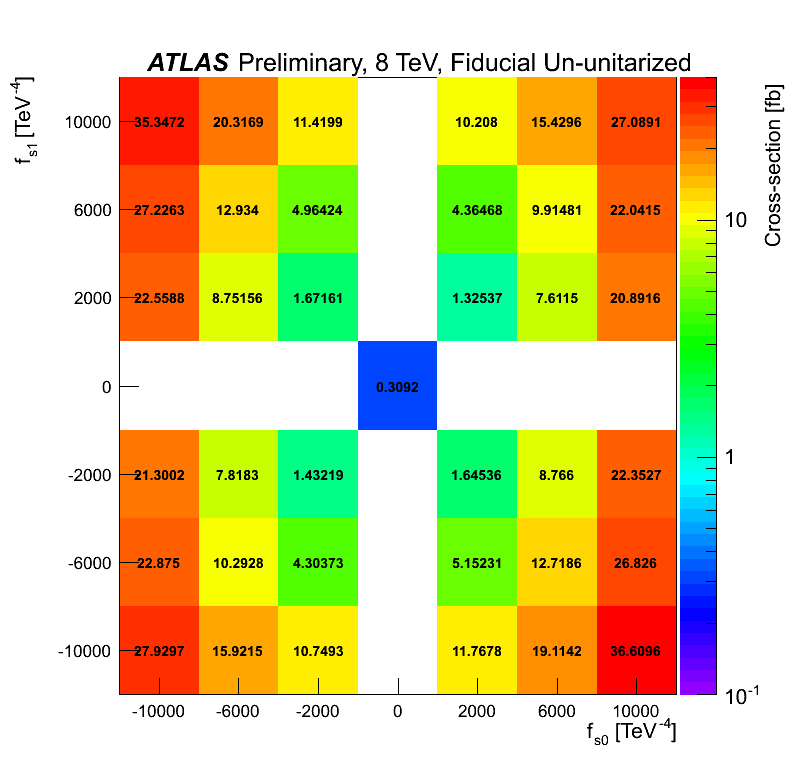
\includegraphics[width=.45\textwidth]{figures/aQGC/fiducial_xsec/www_3l_aqgc_fiducial_ununitarized_noratio.png}
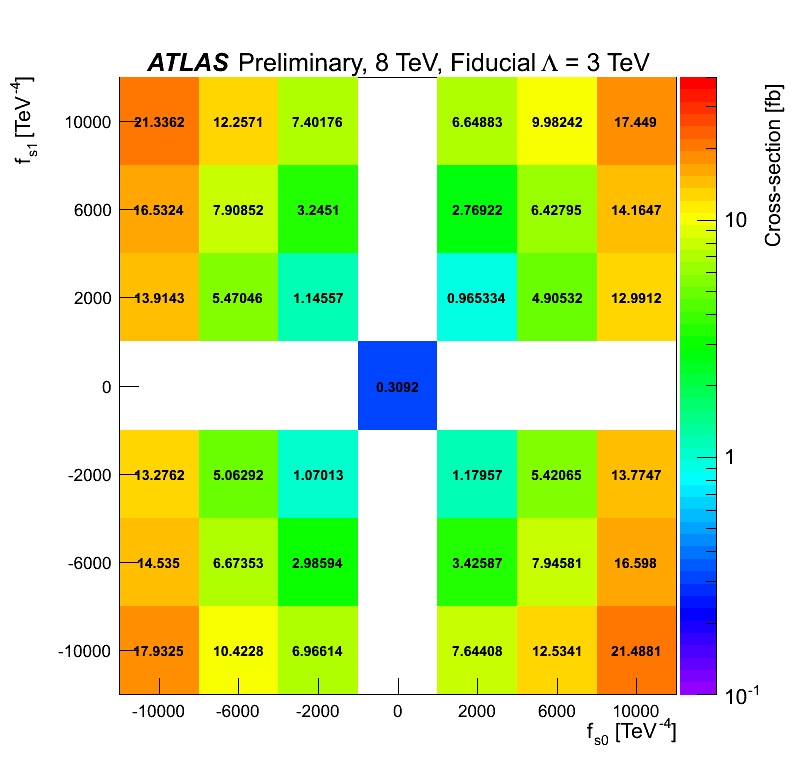
\includegraphics[width=.45\textwidth]{figures/aQGC/fiducial_xsec/www_3l_aqgc_fiducial_3TeV_noratio.png}
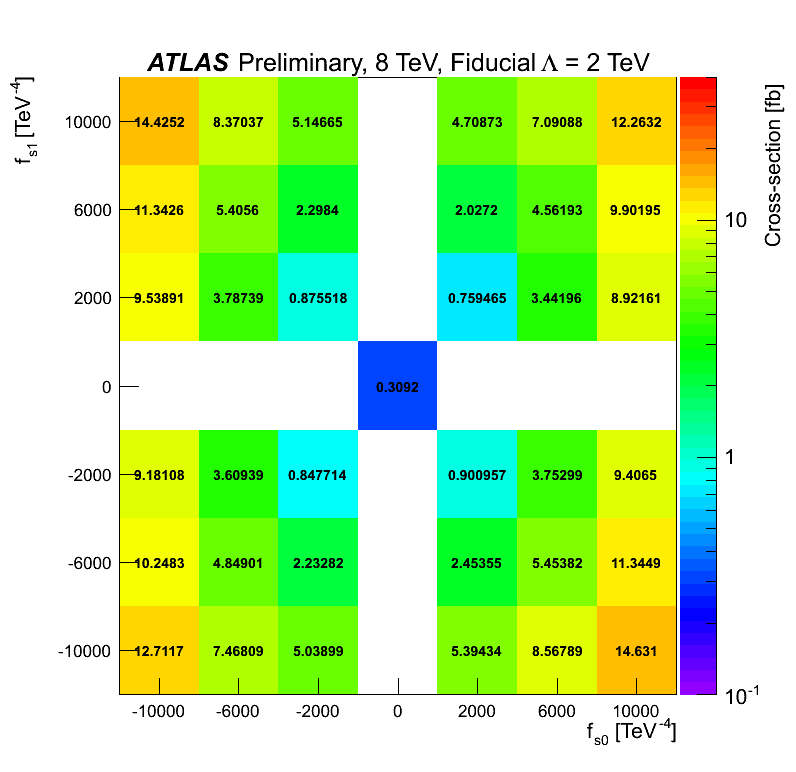
\includegraphics[width=.45\textwidth]{figures/aQGC/fiducial_xsec/www_3l_aqgc_fiducial_2TeV_noratio.png}
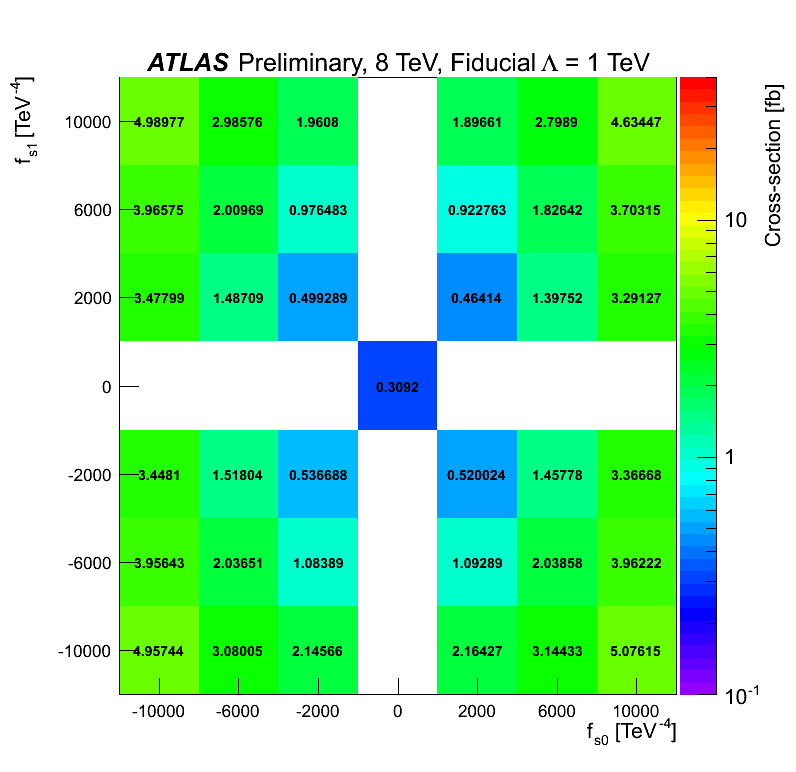
\includegraphics[width=.45\textwidth]{figures/aQGC/fiducial_xsec/www_3l_aqgc_fiducial_1TeV_noratio.png}
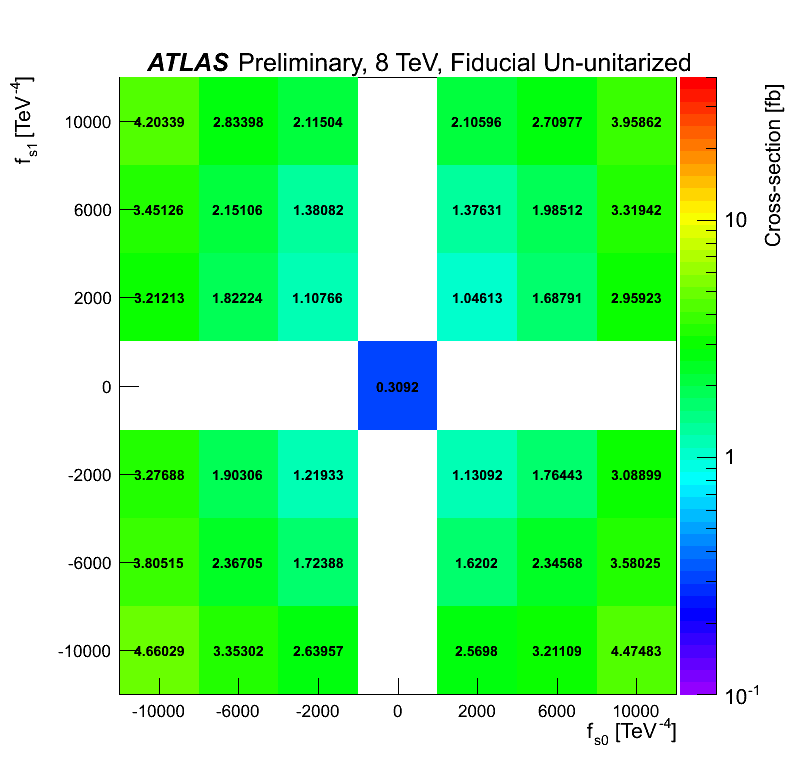
\includegraphics[width=.45\textwidth]{figures/aQGC/fiducial_xsec/www_3l_aqgc_fiducial_p5TeV_noratio.png}
\caption{Fiducial cross-section for unitarized and non-unitarized aQGC signal samples as a function of $f_{s,0}$ vs $f_{s,1}$.
The non-unitarized samples (Top Left) are shown along with the unitarization with 
four different unitarization scales, $\Lambda$: 3~\TeV~(Top Right),
2~\TeV~(Middle Left), 1~\TeV~(Middle Right), and 0.5~\TeV~(Bottom Center).
The total SM cross-section is shown at $f_{s,0}=f_{s,1}=0$ for comparison.}
\label{fig:aqgc_fiducial_xsec_3l}
\end{figure}



The reconstructed number of events were evaluated for the non-unitarized
aQGC signal samples using the same selection as in \sec\ref{sec:signal_regions}.
These values can be used in conjunction with the fiducial cross-sections
to calculate a correction-factor according to \eqn\eqref{eq:cfactor} as a function 
of $f_{s,0}$ and $f_{s,1}$. The correction-factors for the non-unitarized signal samples
are shown averaged over the three signal regions, along with a comparison to the SM point,
in \fig\ref{fig:aqgc_cfactor_3l}.
The correction-factor for the SM point is clearly smaller than that for the aQGC
points by about 40\%. Dedicated studies show that this is a real effect 
that ultimately comes from the aQGC samples having a harder \pt~spectrum
than the SM points and the following two effects:
\begin{itemize}
\item The effect of leptonically decaying $\tau$ leptons is not 
canceled in \eqn\eqref{eq:cfactor}.
\item The electron reconstruction efficiency is strongly \pt~dependent.
\end{itemize}
Note that the harder \pt~spectrum for the aQGC signal samples also 
increases the fiducial cross-sections, but the impact on the correction-factors is more subtle.
The unitarized samples should have a softer \pt~spectrum and thus a
smaller difference between the SM and aQGC correction-factors. However,
reconstructed MC samples were not produced for the unitarized samples.
Instead, we have chosen to use the 
correction-factor for the non-unitarized averaged over the parameter space for 
both the non-unitarized and unitarized samples.  A systematic uncertainty  
is used which is the difference between this averaged non-unitarized
aQGC correction-factor and the SM correction-factor. This should cover all possible differences
in the un-unitarized and unitarized correction-factors.

\begin{figure}[ht!]
\centering
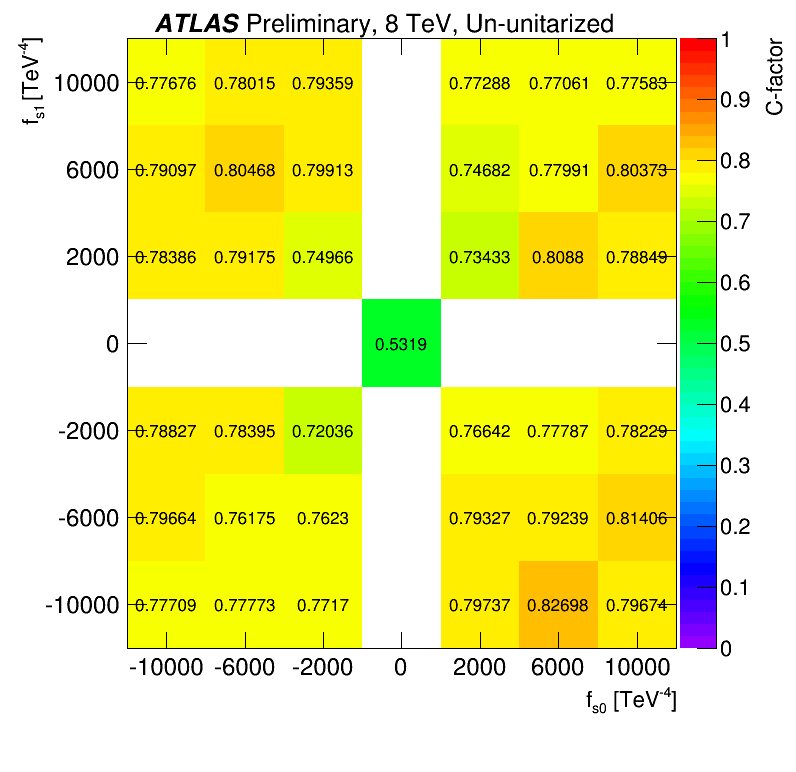
\includegraphics[width=.8\textwidth]{figures/aQGC/cfactor_chargesum.png}
\caption{Correction-factor for non-unitarized aQGC signal samples as a function of $f_{s,0}$ vs $f_{s,1}$.
The SM correction-factor is shown at $f_{s,0}=f_{s,1}=0$ for comparison.}
\label{fig:aqgc_cfactor_3l}
\end{figure}


Once the correction-factors and fiducial cross-sections have been determined,
they can be used to make a prediction on the aQGC signal yield 
for all points.  To allow for interpolation and extrapolation
around the discrete aQGC points evaluated in MC, we also 
fit the predictions using a two-dimensional second order polynomial of 
the form:
\begin{equation}
N_{aQGC}\big(f_{s,0},f_{s,1}\big) = w_0 + w_1 f_{s,0}^2 + w_2 f_{s,1}^2
+ w_3 f_{s,0} + w_4  f_{s,1} + w_5 f_{s,0} f_{s,1}
\end{equation}
where $w_0$ through $w_5$ are the six function parameters in the fit.
%The resulting signal yields and fit functions are shown in \fig\ref{}.




\subsection{Confidence limits on aQGC signal}

The fits of the aQGC signal predictions described above plus the background predictions
from \sec\ref{sec:signal_yield} are input into a likelihood function
in order to extract frequentist 95\% confidence level upper limits on the 
sensitivity to the aQGC signal as observed in the data.
The likelihood function used is of a form similar to \eqn\eqref{eq:poisson_likelihood}
but are determined using software developed within ATLAS \cite{tgclim} that is different
from the one used in \sec\ref{sec:measurement}.
The limits are evaluated either by looking at one aQGC 
parameter at a time, the so-called ``one-dimensional''
limits, or by looking at both aQGC parameters simultaneously, the 
``two-dimensional'' limits. The one-dimensional limits
are presented in \tab\ref{tab:WWW1D}
while the two-dimensional limits are presented in 
\fig\ref{fig:WWW2D}.
  
 
 \begin{table}
   \begin{center}
    \begin{tabular}{  |l| c | c c c | c c c | }
      \hline
      %&$\Lambda$& \multicolumn{6}{c|}{Expected Limit}  \\
      &$\Lambda$& \multicolumn{3}{c|}{Limits on F$_{s0}$ [$10^3~\TeV^{-4}$]}& \multicolumn{3}{c|}{Limits on F$_{s1}$ [$10^3~\TeV^{-4}$]}  \\
      &[\GeV]&  Lower & Upper & Measured & Lower & Upper & Measured  \\
      \hline


\multirow{5}{*}{Expected}	   &500  & -13.61 & 15.38 & ---& -17.69 & 21.02 & ---\\
	   &1000 & -6.03 & 7.31 & ---& -8.32 & 10.05 & --- \\
	   &2000 & -3.46 & 4.48 & --- & -5.04 & 6.27 & --- \\
	   &3000 & -2.82 & 3.83 & --- & -4.15 & 5.34 & --- \\
	   &$\infty$&  -2.18 & 3.14 & --- & -3.35 & 4.27 & --- \\
	   \hline
	   \hline
      
\multirow{5}{*}{Observed}	   &500  & -10.75 & 12.30 & 0.7     $\pm$ 7.5 & -13.16 & 16.07 & 1.34  $\pm$ 8.9 \\
	   &1000 & -4.57 & 5.63 & 0.5          $\pm$ 3.2 & -6.09 & 7.66 & 0.7     $\pm$ 4.1 \\
	   &2000 & -2.50 & 3.49 & 0.5           $\pm$ 1.8 & -3.56 & 4.69 & 0.5     $\pm$ 2.5 \\
	   &3000 & -1.98 & 2.95 & 0.5           $\pm$ 1.5 & -2.89 & 3.96 & 0.5     $\pm$ 2.0 \\
	   &$\infty$ & -1.39 & 2.38 & 0.5 $\pm$ 1.2 & -2.29 & 3.15 & 0.4     $\pm$ 1.6 \\
      \hline
\end{tabular}


     \caption{Expected and observed one-dimensional limits on the aQGC Parameters.
     The non-unitarized case is when $\Lambda=\infty$.}
     \label{tab:WWW1D}

   \end{center}
 \end{table}
 
  % For 2D limits, use Pseudo expected limits are too difficult to achieve for technical issues(can't save results of each pseudo experiment into root file), only width-Test and use-Asimov limits at 95\% CL are shown in Figure.~\ref{fig:WWW2D}.
  % For now, limits shown here are not calculated with up to date signal/background yields and uncertainties, they will be updated in the future and for observed limits, the observed event number is a sum of MC yields, so they are very close to the expected limits, this issue will be modified too.
\begin{figure}[htp]
\centering
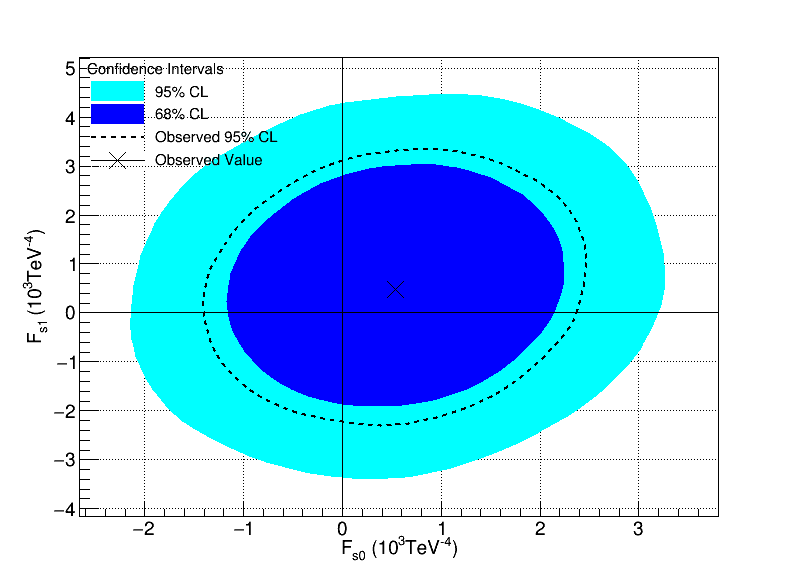
\includegraphics[width=0.45\textwidth]{figures/aQGC/lll-Un-Unit.png}
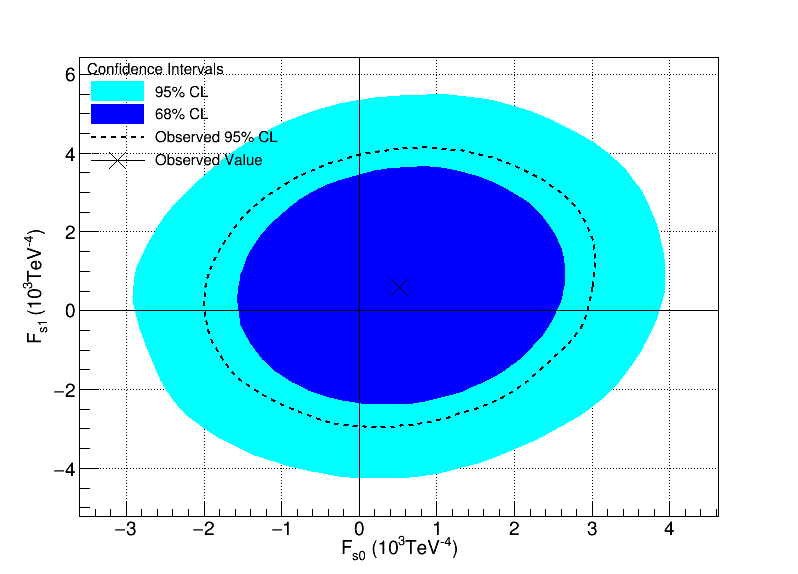
\includegraphics[width=0.45\textwidth]{figures/aQGC/lll-3000.png}
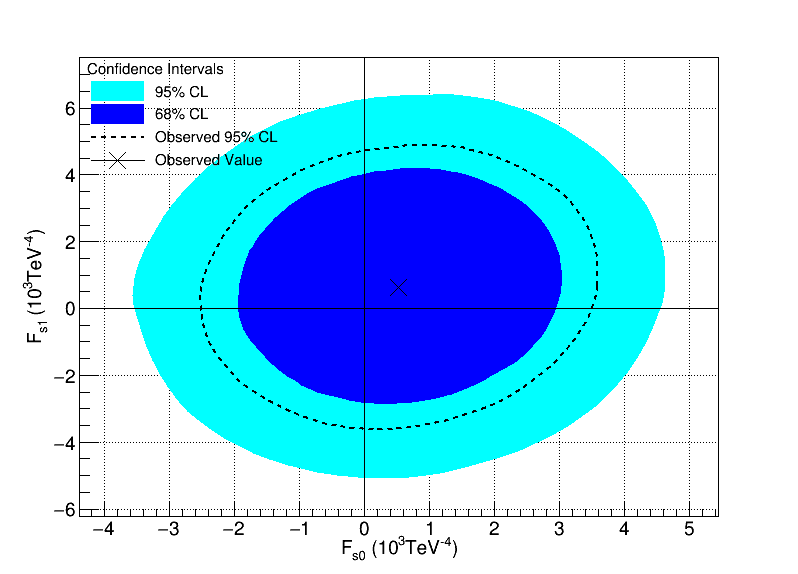
\includegraphics[width=0.45\textwidth]{figures/aQGC/lll-2000.png}
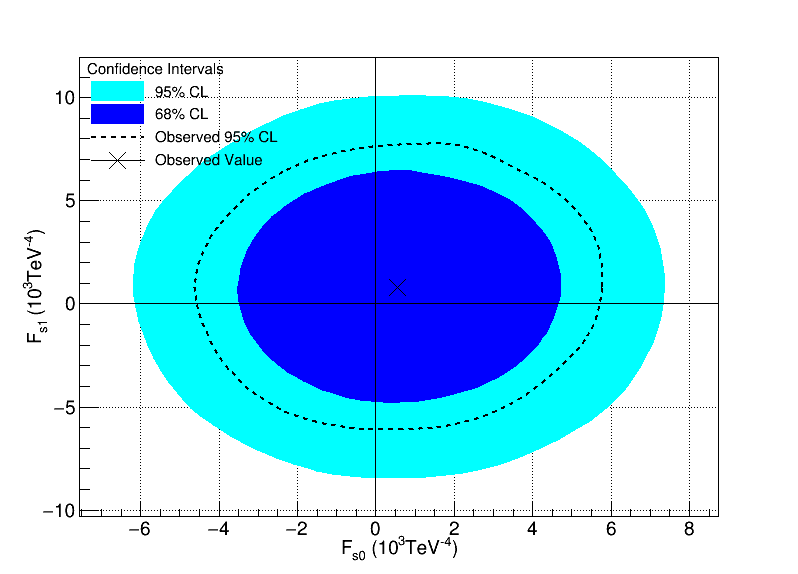
\includegraphics[width=0.45\textwidth]{figures/aQGC/lll-1000.png}
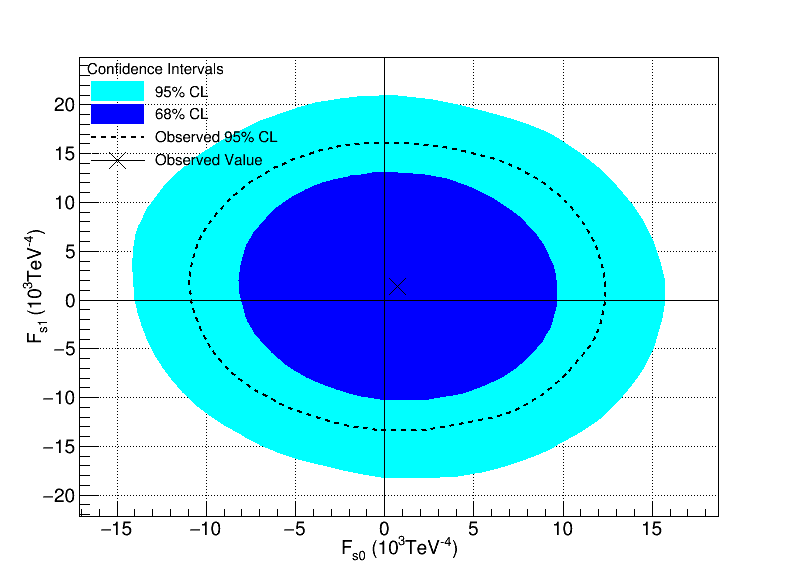
\includegraphics[width=0.45\textwidth]{figures/aQGC/lll-500.png}
\caption{Two-dimensional limits at 95\% CL for the non-unitarized case (Top Left)
and three different choices of the unitarization scale, $\Lambda$:
3~\TeV~(Top Right), 2~\TeV~(Middle Left), 1~\TeV~(Middle Right), and 0.5~\TeV~(Bottom Center).}
\label{fig:WWW2D}
\end{figure}  


  

  

  
